
\begin{frame}{مسئلهٔ فروشندهٔ دوره‌گرد}
\begin{itemize}\itemr
\item[-]
یک فروشندهٔ دوره‌گرد می‌خواهد برای فروش اجناس خود به همهٔ شهرها سفر کند.
هر دو شهر می‌توانند توسط یک جادهٔ یک طرفه به یکدیگر متصل شده باشند و هر جاده طولی معین دارد.
فروشندهٔ دوره‌گرد می‌خواهد از شهر خود سفر را آغاز کند و مسیری را بپیماید که از هر شهر تنها یک بار عبور کند و در پایان به شهر خود بازگردد.
در ضمن می‌خواهد مسیر پیموده شده کوتاهترین مسیر باشد.
\item[-]
این مسئله را با استفاده از یک گراف مدلسازی می‌کنیم.
در یک گراف جهت‌دار، می‌خواهیم کوتاه‌ترین مسیری را پیدا کنیم که از یک رأس آغاز می‌شود، از هریک از رئوس تنها یک بار عبور می‌کند و به رأس اول باز می‌گردد. چنین مسیری یک مسیر بهینه است. از آنجایی که این مسیر بهینه از همهٔ رئوس عبور می‌کند، بنابراین می‌توانیم از هر رأسی مسیر را آغاز کنیم. به مسیری که از هر رأس تنها یک بار عبور می‌کند مسیر همیلتونی می‌گوییم و به مسیری که از هر رأس تنها یک بار عبور کند و به رأس اول بازگردد یک دور همیلتونی می‌گویند. در اینجا به دنبال کوتاهترین دور همیلتونی می‌گردیم.
\end{itemize}
\end{frame}


\begin{frame}{مسئلهٔ فروشندهٔ دوره‌گرد}
\begin{itemize}\itemr
\item[-]
در شکل زیر ماتریس مجاورت برای یک گراف جهت‌دار نشان داده شده است که در آن از هر رأس به رأس دیگر یک یال وجود دارد. اعداد در ماتریس مجاورت طول یال‌ها از یک رأس به رأس دیگرند. کوتاهترین دور همیلتونی در این گراف نشان داده شده است.
\begin{figure}
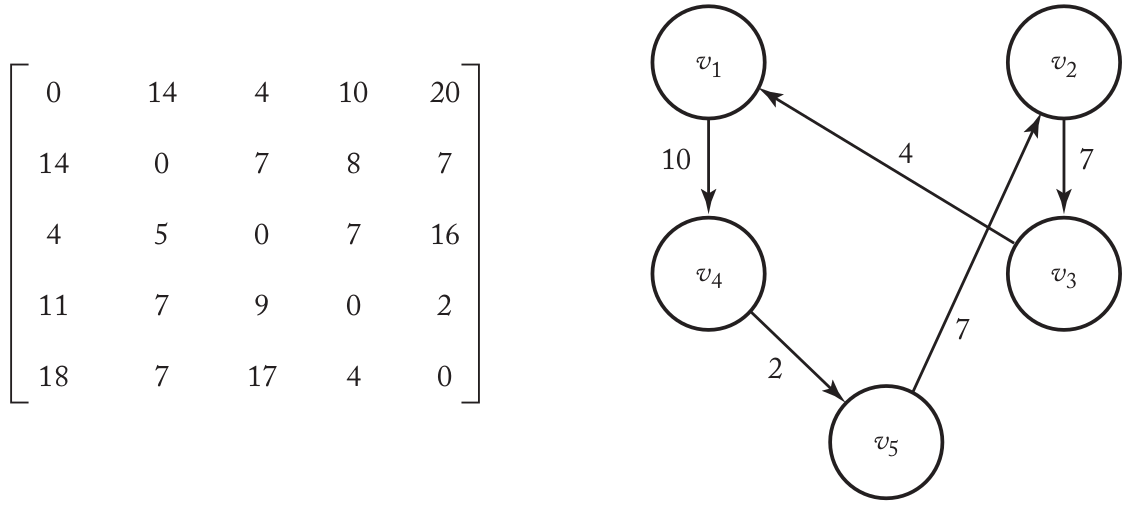
\includegraphics[width=0.7\textwidth]{figs/chap06/263-tsp}
\end{figure}
\end{itemize}
\end{frame}


\begin{frame}{مسئلهٔ فروشندهٔ دوره‌گرد}
\begin{itemize}\itemr
\item[-]
قسمتی از درخت جستجوی فضای حالت برای این مسئله در زیر نشان داده شده است.
\begin{figure}
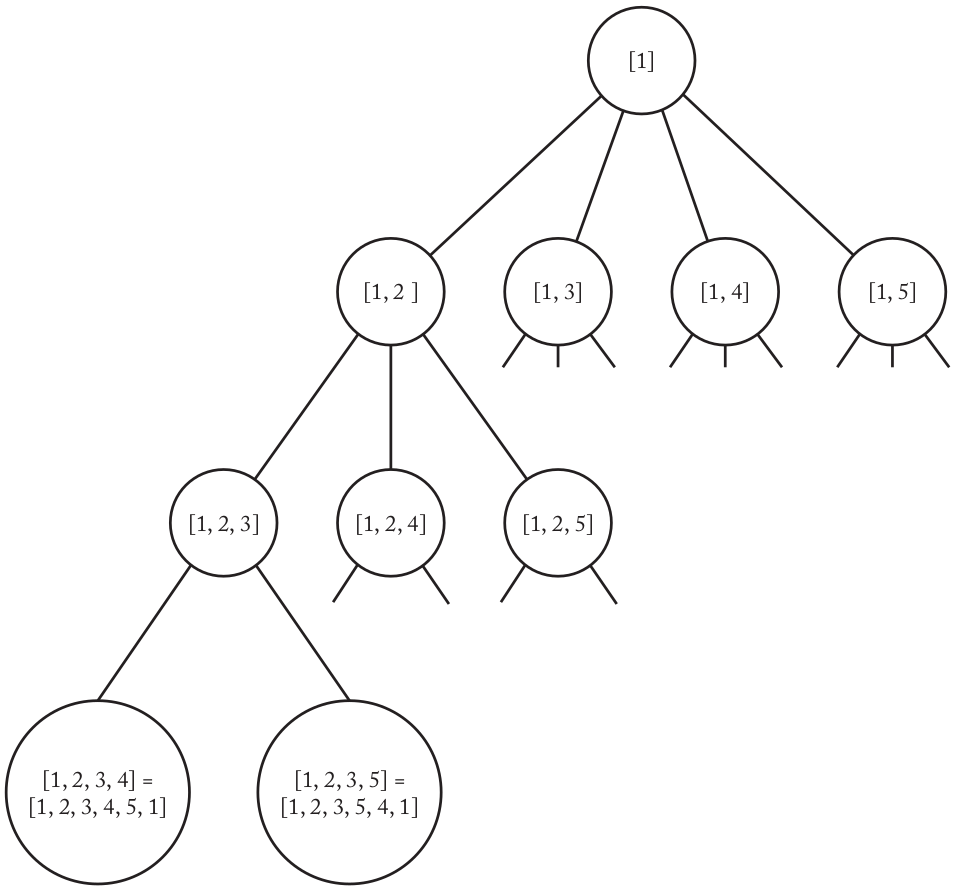
\includegraphics[width=0.5\textwidth]{figs/chap06/264-tsp}
\end{figure}
\end{itemize}
\end{frame}


\begin{frame}{مسئلهٔ فروشندهٔ دوره‌گرد}
\begin{itemize}\itemr
\item[-]
در این درخت فضای حالت، با رأس شماره ۱ از گراف آغاز می‌کنیم. مسیر بهینه ممکن است از هر یک از رئوس ۲ ، ۳ ، ۴ و ۵ عبور کند، بنابراین به ازای هریک از این رئوس یک فرزند در سطح یک در درخت فضای حالت می‌سازیم. رأس
\m{[1,2]}
در درخت فضای حالت مسیری را در گراف مشخص می‌کند که از رأس ۱ و ۲ در گراف عبور کند.
\end{itemize}
\end{frame}


\begin{frame}{مسئلهٔ فروشندهٔ دوره‌گرد}
\begin{itemize}\itemr
\item[-]
اکنون باید برای هر رأس در درخت فضای حالت یک مقدار کران پیدا کنیم. در هر رأس درخت فضای حالت یک کران پایین برای طول مسیری که می‌توان با بسط دادن آن رأس به دست آورد محاسبه می‌کنیم.
\item[-]
اگر کران پایین محاسبه شده در یک رأس از کوتاهترین مسیر همیلتونی به دست آمده تا آن لحظه کمتر باشد، آن رأس درخت فضای حالت امیددهنده است و آن رأس را بسط می‌دهیم، در غیر اینصورت آن رأس نومیدکننده است و بسط دادن را از آن رأس ادامه نمی‌دهیم.
\end{itemize}
\end{frame}


\begin{frame}{مسئلهٔ فروشندهٔ دوره‌گرد}
\begin{itemize}\itemr
\item[-]
برای محاسبهٔ کران به صورت زیر عمل می‌کنیم.
\item[-]
در هر رأس درخت فضای حالت تعدادی از رئوس گراف پیمایش شده و تعدادی پیمایش نشده‌اند.
به ازای رأس‌های پیمایش شده در گراف طول مسیر معین شده است. اما به ازای رأس‌های پیمایش نشده در گراف باید یک کران پایین برای طول مسیر محاسبه کنیم.
\item[-]
رأس پیمایش نشدهٔ
\m{V_i}
را در نظر بگیرید. جهت پیدا کردن یک کران پایین برای کوتاهترین مسیر،
به ازای هریک از رأس‌های پیمایش نشدهٔ
\m{V_i}
باید کوتاهترین یال خروجی از آن رأس را به صورت
\m{\min_{k} (V_i,V_k)}
 محاسبه کنیم و طول کوتاهترین یال‌های خروجی را به ازای همهٔ رئوس پیمایش نشده به صورت
\m{\sum_{i} \min_{k} (V_i,V_k)}
محاسبه کنیم.
\item[-]
 به عبارت دیگر به ازای هر یک از رئوس پیمایش نشدهٔ
\m{V_i}
باید یالی را پیدا کنیم که از
\m{V_i}
خارج می‌شود و کمترین هزینه را دارد.
مجموع طول این یال‌ها یک کران پایین برای طول مسیر است.
توجه کنید که این بدین معنا نیست که کوتاهترین‌ها الزاما در مسیر همیلتونی انتخاب می‌شوند، بلکه بدین معناست که هیچ مسیر همیلتونی با طول کمتر از مقدار محاسبه شده وجود نخواهد داشت.
\end{itemize}
\end{frame} 


\begin{frame}{مسئلهٔ فروشندهٔ دوره‌گرد}
\begin{itemize}\itemr
\item[-]
محاسبه کران را با یک مثال بررسی می‌کنیم. ماتریس مجاورت زیر را در نظر بگیرید.
\begin{figure}
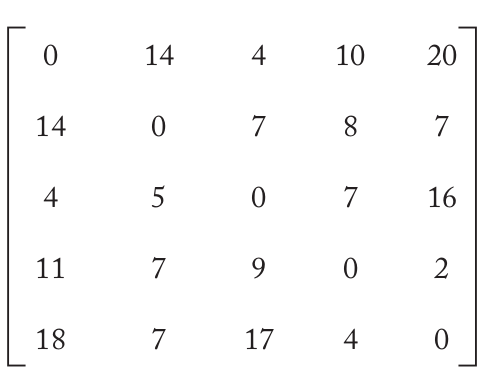
\includegraphics[width=0.2\textwidth]{figs/chap06/263-tsp-matrix}
\end{figure}
\item[-]
در ریشه درخت فضای حالت هیچ‌یک از رئوس گراف پیموده نشده‌اند. کران پایین مسیر در ریشه را می‌توانیم توسط رابطهٔ
\m{\sum_i \min_k (V_i,V_k)}
محاسبه کنیم. این مقدار برابراست با :
\begin{align*}
\m{\sum_i \min_k (V_i,V_k) = 4 + 7 + 4 + 2 + 4 = 21}
\end{align*}
\item[-]
بنابراین طول کوتاه‌ترین مسیر ممکن با شروع از رأس 
\m{V_1}
برابر است با ۲۱ .
\end{itemize}
\end{frame} 

\begin{frame}{مسئلهٔ فروشندهٔ دوره‌گرد}
\begin{itemize}\itemr
\item[-]
حال به ازای همهٔ فرزندان ریشه یک کران محاسبه می‌کنیم.
%و رأسی را برای پیمایش انتخاب می‌کنیم که کران محاسبه شده برای آن کمینه باشد.
برای مثال
 رأس
\m{[1,2]}
در درخت فضای حالت را در نظر بگیرید. یالی با طول
\m{14}
از رأس
\m{V_1}
به رأس
\m{V_2}
پیموده شده است.
طول کوتاهترین مسیری که با ادامهٔ این مسیر می‌تواند وجود داشته باشد برابر خواهد بود با ۱۴ به علاوه کوتاهترین مسیری که از بقیه رئوس به غیر از 
\m{V_2}
 عبور می‌کند. توجه کنید که از آخرین رأس در مسیر که در اینجا
\m{V_2}
است،
نمی‌توانیم به اولین رأس در مسیر که در اینجا
\m{V_1}
است،
بازگردیم اما امکان این که از هر یک از رئوس دیگر به 
\m{V_1}
برویم وجود دارد.
\begin{figure}
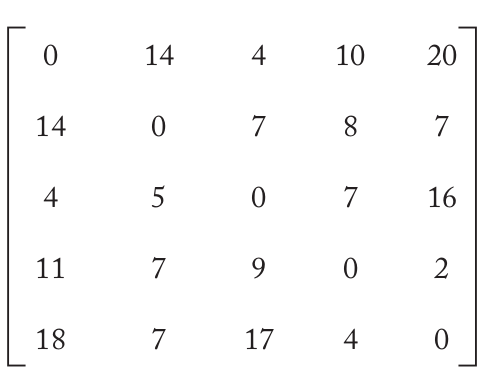
\includegraphics[width=0.2\textwidth]{figs/chap06/263-tsp-matrix}
\end{figure}
\item[-]
 کران پایین مسیر در این رأس برابراست با :
\begin{align*}
\m{14 + \sum_{i\in \{2,3,4,5 \}} min_k(V_i,V_k) = 14 + 7 + 4 + 2 + 4 = 31}
\end{align*}
\end{itemize}
\end{frame} 


\begin{frame}{مسئلهٔ فروشندهٔ دوره‌گرد}
\begin{itemize}\itemr
\item[-]
بدین ترتیب می‌توانیم مقدار کران را در هر‌یک از رئوس درخت فضای حالت به صورت زیر محاسبه کنیم.
\begin{figure}
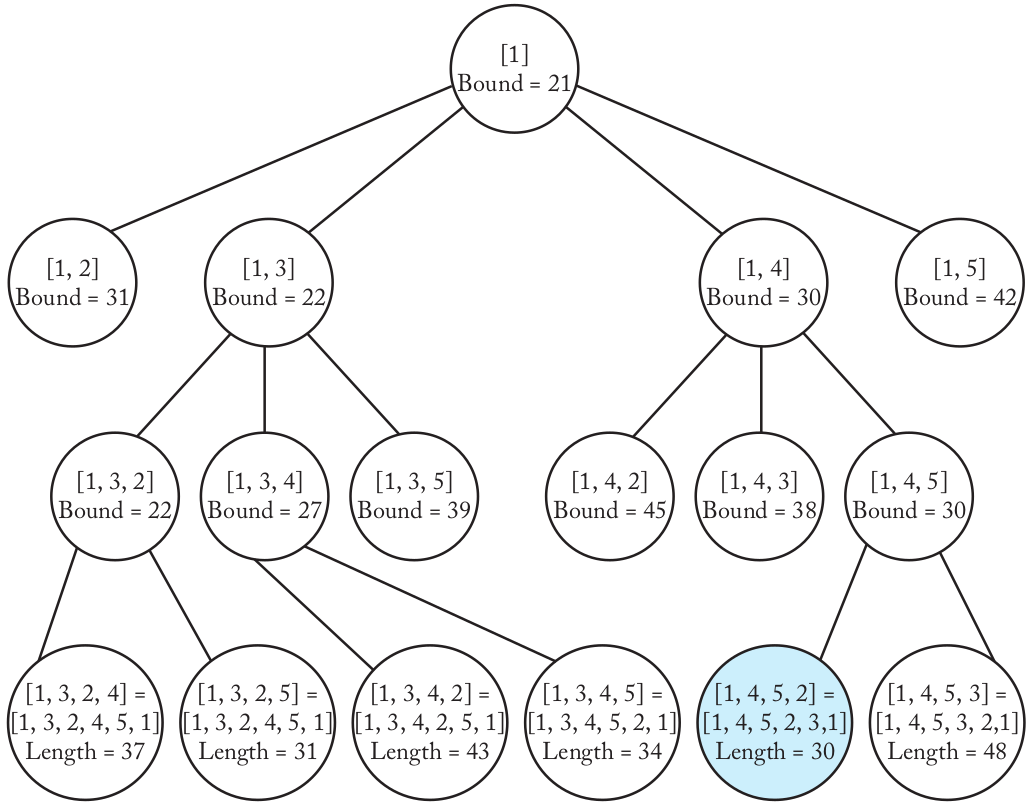
\includegraphics[width=0.5\textwidth]{figs/chap06/267-tree}
\end{figure}
\end{itemize}
\end{frame} 


\begin{frame}{مسئلهٔ فروشندهٔ دوره‌گرد}
\begin{itemize}\itemr
\item[-]
مقدار کران را برای همهٔ رئوس محاسبه می‌کنیم و رأسی را برای بسط دادن انتخاب می‌کنیم که مقدار کران آن کمینه باشد.
\item[-]
در اینجا از بین رئوس
\m{[1,2], [1,3], [1,4], [1,5]}
رأس 
\m{[1,3]}
کوچکترین کران را دارد که برابر با ۲۲ است.
\item[-]
وقتی رأس 
\m{[1,3]}
بسط داده شد، در نهایت کوتاهترین طول مسیری که در ریشه به دست می‌آید برابر با ۳۱ است.
\item[-]
اما در رأس 
\m{[1,4]}
همچنان یک کران کوچکتر برابر با ۳۰ وجود دارد،‌ بنابراین آن رأس را بسط می‌دهیم و در نهایت مسیری با طول ۳۰ پیدا می‌کنیم.
\end{itemize}
\end{frame} 


\begin{frame}{مسئلهٔ فروشندهٔ دوره‌گرد}
\begin{itemize}\itemr
\item[-]
هر رأس در درخت فضای حالت را می‌توانیم با ساختمان زیر نشان دهیم.
\begin{algorithm}[H]\alglr
\caption{Node Structure} 
\begin{algorithmic}[1]
\Statex \textbf{struct} node
\State~~ int level \LeftComment{the node’s level in the tree}
\State~~ ordered-set path
\State~~ int bound
\end{algorithmic}
\label{alg:node-structure}
\end{algorithm}
\end{itemize}
\end{frame} 


\begin{frame}{مسئلهٔ فروشندهٔ دوره‌گرد}
\begin{itemize}\itemr
\item[-]
در الگوریتم زیر برای یک گراف با n رأس، که وزن یال‌های آن با ماتریس W داده شده است، می‌خواهیم کوتاهترین دور همیلتونی را پیدا کنیم.
\begin{algorithm}[H]\alglr
  \caption{Travelling Salesman Problem} 
  \begin{algorithmic}[1]
   \Func{Travelling-Salesman-Problem}{int n, int-matrix W}
   \State ordered-set opttour \LeftComment{Optimal tour}
   \State int minlength = $\infty$ \LeftComment{The length of the optimal tour}
   \State priority-queue PQ
   \State node v
   \State initialize(PQ)		\LeftComment{Initialize PQ to be empty.}
   \State v.level = 0
   \State v.path = [1]	\LeftComment{Make first vertex the}
   \State v.bound = bound(v)		\LeftComment{starting one.}
   \State insert(PQ,v)                           
  \end{algorithmic}
  \label{alg:tsp1}
\end{algorithm}
\end{itemize}
\end{frame} 


\begin{frame}{مسئلهٔ فروشندهٔ دوره‌گرد}
\begin{center}
\resizebox{.74\textwidth}{!}{
\begin{minipage}{\textwidth}
\begin{algorithm}[H]\alglr
  \caption{Travelling Salesman Problem} 
  \begin{algorithmic}[1]
  \setcounter{ALG@line}{9}
  % \Func{Travel2}{int n, const number W[] [], ordered-set\& opttour, number\& minlength}
   \While{!empty(PQ)}
   	  \State remove(PQ, v)\LeftComment{Remove node with best bound.}
   	  \If{(v.bound < minlength)}
   			   \For{(all i not in v.path)}
   			           %\State create new node u
   			           \State create the new tree node u
   			           \State u.level = v.level + 1\LeftComment{Set u to a child of v.}
   					   \State u.path = [v.path , i] \LeftComment{put i at the end of v.path}
						\Statex \LeftComment{Check if next vertex completes a tour.}   					   
   					   \If{(u.level == n-2)}
							\Statex \LeftComment{put the last vertex not in u.path and also vertex 1 at the end of u.path}   					       
   					        \State u.path = [u.path, last-vertex, 1]
                           \Statex \LeftComment{Function length computes the length of the tour.}   							
   							\If{(length(u) < minlength)}
   									\State minlength = length(u)
   									\State opttour = u.path
   							\EndIf
   					   \Else
   							\State u.bound = bound(u)
   					        \If{(u.bound < minlength)}
   							   \State insert(PQ, u)
   					         \EndIf
   					   \EndIf
   		   \EndFor
   	   \EndIf
   \EndWhile     
   \State \Return (opttour, minlength)                         
  \end{algorithmic}
  \label{alg:tsp2}
\end{algorithm}
\end{minipage}
}
\end{center}
\end{frame}



\begin{frame}{مسئلهٔ فروشندهٔ دوره‌گرد}
\begin{itemize}\itemr
\item[-]
کران یک رأس درخت فضای حالت را به صورت زیر محاسبه می‌کنیم.
\begin{center}
\resizebox{.8\textwidth}{!}{
\begin{minipage}{\textwidth}
\begin{algorithm}[H]\alglr
\caption{Computing Bound for Travelling Salesman Problem} 
  \begin{algorithmic}[1]
   \Func{bound}{node v}
   \State bound = 0  
   \For{edge (i,j) in v.path}
       \State bound += length(i,j)
   \EndFor  
   %\State min = $\infty$
   \State i = last vertex in v.path
   \State min = $\min_k$ \{ W[i][k], vertex k $\not\in$ v.path \}
   %\For{vertex k not in v.path}
   %        \If{W[i][k] < min}
   %            \State min = W[i][k]
   %        \EndIf
   %    \EndFor  
   \State bound += min      
   \For{vertex i $\not\in$ v.path}
   \State min = $\min_k$ \{ W[i][k], vertex k $\not\in$ v.path \textbf{or} k = 1 \}
       %\State min = W[i][1]
       %\For{vertex k not in v.path}
       %    \If{W[i][k] < min}
       %        \State min = W[i][k]
       %    \EndIf
       %\EndFor
       \State bound += min
  \EndFor
  \State \Return bound
  \end{algorithmic}
  \label{alg:tsp-bound}
\end{algorithm}
\end{minipage}
}
\end{center}
\end{itemize}
\end{frame} 

\iffalse
\begin{frame}{مسئلهٔ فروشندهٔ دوره‌گرد}
\begin{itemize}\itemr
\item[-]
ممکن است در یک الگوریتم شاخه و کران بتوانیم چندین تابع کران پیدا کنیم که در این موارد معمولاً یکی از توابع، کران بهتری پیدا می‌کند.
\end{itemize}
\end{frame}
\fi
